\documentclass[a4paper, 12pt]{extarticle}
\usepackage[utf8]{inputenc}

\usepackage{float}
\usepackage{graphicx}
\usepackage{hyperref}
\usepackage{parskip}
\usepackage{booktabs}
\usepackage{caption}

\usepackage{biblatex}
\addbibresource{main.bib}
\addbibresource{gsa.bib}


% >= 3.45cm is too large to fit 2 names per row
\usepackage[left=2cm,right=2cm]{geometry}


\title{
    CITS4404 Team Project - Building AI Trading Bots
    \\ \large Group 6 - Part I 
}
\author{
    Chen, Zijian\\
    \normalsize \texttt{22998691@student.uwa.edu.au}
    \and
    Dai, Ethan\\
    \normalsize \texttt{23625929@student.uwa.edu.au}
    \and
    Ida Bagus Prawira Janottama Kn\\
    \normalsize \texttt{23894575@student.uwa.edu.au}
    \and
    Nadeesha Adikari\\
    \normalsize \texttt{24041382@student.uwa.edu.au}
    \and
    Su, Daniel\\
    \normalsize \texttt{22965999@student.uwa.edu.au}
    \and
    Townshend, Nathan\\
    \normalsize \texttt{22970882@student.uwa.edu.au}
}
\date{\today}

\begin{document}

\clearpage

\maketitle


\newpage
\tableofcontents


\newpage
\section{Introduction}\label{sec:intro}
% \input{introduction}


\newpage
\section{Gravity Search Algorithm}\label{sec:alg:gsa}
The Gravitational Search Algorithm (GSA) \cite{GSA} was introduced in 2009, developed as another option for non-linear optimisation.
Where the majority of nature-based optimisation algorithms use multiple agents with some form of swarm intelligence to perform exploration of the search space and exploitation of found maximums, GSA uses multiple agents but with rules based on Newtonian gravity and motion.

In GSA, Gravitational forces are applied on and between agents in the search space, with the mass of an agent is based on its fitness compared to the other agents (a more fit agent is more massive).
Agents are initially randomly distributed throughout the search space.
The new velocity (and hence position) of an agent at each time step is calculated by randomly retaining a portion of the previous velocity, and applying any acceleration due to gravity.
The force due to gravity and the total number of agents can be modified over time steps, for example to have lower initial gravity to promote early exploration, or to reduce the number of agents later on to simplify the system and promote exploitation.
While Newtonian gravity has masses attracted inversely proportional to the square of their distance (with $F \propto \frac{1}{R^2}$), the original paper on GSA has the force inversely proportional to their distance ($F \propto \frac{1}{R}$).
Different implementations and versions of the GSA algorithm use either $R$ or $R^2$ - for example of the two papers discussed below, GGSA uses $R$, and EGSA uses $R^2$.


\subsubsection{Motivation for improvements to GSA}\label{sec:alg:gsa:motiviation}
While GSA performed better in accuracy and convergence speed on benchmarks than other popular algorithms of the time such as PSO and Real Genetic Algorithm \cite{GSA}, there are a number of issues that have lead to modified versions of GSA being proposed and utilised.

The two phases of these nature-inspired algorithms - exploration and exploitation - generally conflict, with increasing the performance of an algorithm in one phase generally weakening the performance in the other.
To combat this, hybrid algorithms combining multiple optimisation algorithms have been tested, for example SA-PSO (see Section \ref{sec:alg:sa-pso} of this report) that uses Simulated Annealing to improve the exploitation performance of the PSO algorithm.
However, while combining multiple algorithms this way improves performance, it can come at the cost of considerable additional computation, potentially even greater than the sum of running each algorithm sequentially.
GSA is an effective optimisation algorithm for large-scale problems, as it is able to perform effectively with a significantly smaller agent count than other algorithms such as PSO \cite{EGSA}, however it is not exempt from the trade-off of exploration vs exploitation.
Local search has been suggested as a way to improve its exploitation \cite{GSA}, but is also computationally expensive particularly in higher dimensional search spaces.
Thus, significant improvements able to be made to the exploration and exploitation performance of algorithms with minimal additional computational power would be of interest for large-scale problems where it might be infeasible to use hybrid algorithms or local search.


\subsubsection{Enhanced GSA}\label{sec:alg:gsa:egsa}
Optimal Power Flow (OPF) for electrical grids is a large-scale optimisation problem of obvious interest to reduce operational costs, network losses, and environmental pollution.
It has a discontinuous, nonlinear, and very large solution space making it difficult or infeasible to utilise some optimisation algorithms.
Enhanced GSA (EGSA) was proposed by Jahan and Amjady \cite{EGSA} in 2013 to improve on the exploration of GSA, particularly for a problem with such a large solution space.
The key modification in EGSA is the introduction of a 'mutation' operator, which continuously generates new agents throughout the solution space.
When a mutation is performed, up to half of the worst agents are randomly selected, and a random number of their variables (position within a particular dimension) are changed to random values.
Initially the random values can be from anywhere in that dimension to assist with exploring the entire solution space early on, with the size of the possible change being restricted and reduced as the number of iterations increase to support convergence later on in the search.

To evaluate the proposed algorithm, the paper selected a number of standard OPF optimisation algorithms (Genetic Algorithm, Differential Evolution, PSO, and GSA).
Each algorithm, along with EGSA, were then benchmarked using 5 sample problems - 4 standard but small OPF IEEE datasets, and an additional less standard but significantly larger dataset.
Each algorithm was given 100 agents and 1000 iterations.
While GSA consistently performed well, EGSA outperformed all other algorithms on all sample problems - both with more optimal results, and requiring less compute time.
Additionally, EGSA was the only algorithm that found a solution for the large dataset that was actually economically viable to utilise.

% TODO conclusion


\subsubsection{GGSA}\label{sec:alg:gsa:ggsa}
As the number of iterations of GSA increase agents all increase in mass, therefore slowing down the overall exploitation and search due to increased inertia - Mirjalili and Lewis \cite{GGSA} proposed gbest-guided GSA (GGSA) in 2014 as a computationally cheap way to combat this and improve the exploitation of GSA.
GSA can additionally struggle during exploitation when a number of agents in a neighbourhood are attracted to each other and not necessarily able to accelerate towards a nearby optimum.
% * Figure not included to save space given the 2-page restriction
% An additional problem with GSA during exploitation is demonstrated in Figure \ref{fig:alg:gsa:neighbourhood-problem}, where agents in a neighbourhood are attracted to each other and not necessarily able to accelerate towards a nearby optimum.

% \begin{figure}[H]
%     \centering
%     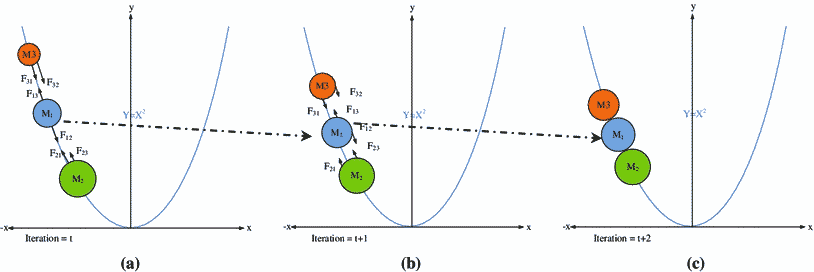
\includegraphics[width=0.8\linewidth]{figures/gsa_neighbourhood_problem.png}
%     \caption{Movement behaviour of neighbourhood near an optimum, Figure 1 from \cite{GGSA}}
%     \label{fig:alg:gsa:neighbourhood-problem}
% \end{figure}

GGSA addresses these two issues by introducing an additional force - a 'global best' solution is kept track of and updated each iteration, and agents are attracted to this 'gbest' solution in the same way they are attracted to the masses of the other agents.
To prevent this from having a significant detrimental effect to early exploration, the gravitational force towards the other agents and the gravitational force towards the gbest solution are weighted separately, with the agent force prioritised during the exploration stage and dropping off as the gbest force is increasingly prioritised during the exploitation stage.

% TODO cover GGSA results

% TODO GGSA conclusion


% Ethan's section
\newpage
\section{Modified Particle Swarm Optimisation with Simulated Annealing}

\subsection{Particle Swarm Optimisation}

Particle Swarm Optimisation (PSO) was first introduced by Kennedy and Eberhart \cite{kennedy1995particle} in 1995 as a method for optimisation in continuous nonlinear search spaces. It was inspired by the swarming social behaviour exhibited naturally by species such as fish or birds. The motivation for mimicking nature in this particular way was the observation that individual members in flocks benefit from the collective experiences of all other members \cite{wilson2000sociobiology}. An example could be birds flocking to a food source, many individuals within the flock would have no prior knowledge of the location of a new food source but the information spreads to all individuals through flocking behaviour. 

The original PSO algorithm operated on several basic rules for each individual within the swarm. Using some cost function, each individual remembered its own personal best (pbest) position and also knows the global best (gbest) position found by any individual within the swarm.

The velocity update of an individual depends on its distance relative to both pbest and gbest with hyperparameters p\_increment and g\_increment determining the magnitude of the velocity increase towards either point. The resulting velocity update is a vector addition of the velocity towards pbest and gbest.


\subsection{Motivating Particle Swarm Optimisation with Simulated Annealing}

Particle Swarm Optimisation with Simulated Annealing (SA-PSO) was introduced by Shieh et al. \cite{shieh2011modified} to address two optimisation issues at the time of publishing.

\begin{enumerate}
    \item Genetic Algorithms (GA) struggled with epistasis where genes were highly correlated with each other within the chromosome causing issues with crossover for new generations. It was also more computationally inefficient compared to PSO.
    \item PSO struggled with premature convergence to local minima due to localisation of the particles. Due to the attraction to pbest and gbest, exploration is largely discouraged in the algorithm.
\end{enumerate}

Simulated Annealing (SA) provides an exploration property using the metropolis process, which converges asymptomatically to the global optimum given certain preconditions. A novel SA and PSO hybrid approach is proposed due to the computational efficiency of PSO compared to other optimisation algorithms and the more stable convergence properties of SA stemming from the algorithm’s greater ability to explore the search space.

A high initial temperature increases the acceptance probability for new (poorer) solutions, increasing the randomness of velocity updates leading to a larger subset of the search spacing being explored by particles. To stabilise the initial iterations, elitism (a concept from Genetic Algorithms where the top performing individuals are preserved into the next generation) for optimal solutions is maintained. As temperature drops, the swarm begins to converge more strongly onto gbest to perform exploitation of the known solutions in the search space.

\subsection{Method and Results}

The SA-PSO algorithm contains 6 hyperparameters that require tuning before being applied to the benchmark functions. This is performed through a coarse exhaustive search of all potential values within a range. For example, the initial temperature value was tested for between 50 and 90 in increments of 10.

The proposed SA-PSO algorithm and baseline GA, SA and PSO algorithms are then benchmarked on a selection of test functions with various dimensionality mostly taken from mathematics and physics such as the Zakharov function. The indicator used for performance is the rate of obtaining the optimal solution.

Each algorithm was run on each benchmark function 100 times. The final performance metric comparing SA-PSO to its predecessor algorithms is the average rate of obtaining the optimal solution.

The new algorithm demonstrated a significant performance improvement over the second-best algorithm PSO at an average convergence rate of 98.7\% compared to 92.5\%.

The consistency of the algorithms were also demonstrated through the mean value of the solution obtained over the 100 runs for each benchmark function. SA-PSO demonstrated means which were closest to the known optimum on the vast majority of benchmarks demonstrating the stability of convergence of the algorithm.

\subsection{Discussion}

The paper concluded that SA-PSO demonstrated strong results as a consequence of combining the explorative nature of SA to counteract the tendency of PSO to fall into local extrema. The performance justifies the claim that that SA-PSO is a capable optimisation algorithm for non-linear optimisation problems. 
However, the benchmark functions were all continuous and well-defined functions. The performance of SA-PSO on real-world data cannot be extrapolated from this paper as it may not be differentiable or continuous.

% Nadeesha's section
\newpage
\section{Grey Wolf Optimizer}
The Grey Wolf Optimizer (GWO) aims to overcome key limitations in existing optimization algorithms, such as getting trapped in local optima, poor convergence behaviour, and an imbalance between exploration and exploitation. While algorithms like Particle Swarm Optimization (PSO), Gravitational Search Algorithm (GSA), and Differential Evolution (DE) have been successful in many scenarios, they often struggle with these issues. GWO addresses them by mimicking the social hierarchy and hunting strategies of grey wolves, leading to a more adaptive and balanced search process. The algorithm's structure, based on four types of wolves: alpha ($\alpha$), beta ($\beta$), delta ($\delta$), and omega ($\omega$), enhances its ability to explore the search space globally and exploit promising regions effectively\cite{mirjalili2014grey}.

\subsection{Limitations of Previous Approaches}
The paper \cite{mirjalili2014grey} highlights that metaheuristic techniques tend to outperform classical heuristics due to their simplicity, ability to avoid local optima, flexibility across different problem domains without structural changes, and their derivative-free approach that enables the process to begin from a random solution. Moreover, population-based algorithms have shown significant advantages over single-solution-based approaches.

GWO is a metaheuristic, population-based, swarm intelligence algorithm inspired by the social hierarchy and hunting behaviour of grey wolves. However, many existing algorithms still face critical challenges. A major issue is local optima trapping, where the algorithm prematurely settles on suboptimal solutions. Another significant challenge is the lack of balance between exploration and exploitation, some algorithms overexploit early good solutions and fail to adequately explore the broader search space, especially due to their stochastic behaviour. Furthermore, slow or improper convergence is also a limitation, as some algorithms struggle to efficiently reach high-quality solutions due to weak search strategies.These limitations have motivated the development of the GWO, which seeks to address these deficiencies through a more effective and biologically inspired approach. 

\subsection{Introduction of the Novel Idea}
Although many earlier swarm intelligence (SI) algorithms were inspired by natural hunting or search behaviors, they often overlooked the internal leadership dynamics within animal groups. The Grey Wolf Optimizer (GWO) introduces a novel idea by simulating the leadership hierarchy and social behaviour of grey wolves. It categorizes the population into four types of wolves, alpha ($\alpha$), beta ($\beta$), delta ($\delta$), and omega ($\omega$), to represent the hierarchy of decision-making. The alpha wolf represents the current best solution, the beta and delta are the second and third best, while the remaining candidates are considered omega wolves.

The algorithm also mimics the three main phases of hunting: searching for prey, encircling prey, and attacking prey. These behaviors guide the population’s movement in the search space, with the alpha, beta, and delta wolves influencing the search direction. This structured yet dynamic mechanism allows the GWO algorithm to maintain a high degree of randomness and diversity, helping it to avoid local optima. \cite{kandasamy2020literature}

\subsection{Demonstration of the New Approach}
The new approach is demonstrated through benchmarking experiments on 29 test functions. Among these, 23 are classical benchmark functions, and the remaining 6 are composite benchmark functions. These functions are used to evaluate the algorithm’s performance in terms of exploration, exploitation, and local optima avoidance. Unimodal functions are used for exploitation analysis, multimodal functions for exploration analysis, and composite benchmark functions for local minima avoidance analysis. The algorithm was run 30 times for each benchmark, and statistical results (average and standard deviation) were compared to other popular swarm intelligence algorithms.   Additionally, the GWO algorithm is applied to three classical engineering design problems: tension design, welded beam design, and pressure vessel design. It was also tested on a real-world optical buffer design problem, running the algorithm 20 times to validate its ability to solve real-world problems with constraints. \cite{mirjalili2016multi}.

\subsection{Results and Validation}
The performance of GWO was validated through benchmarking against well-known optimization algorithms, such as PSO, GSA, and GA, across various test functions, including unimodal, multimodal, and composite functions. Statistically significant improvements were observed in key metrics such as Delay-Bandwidth Product (DBP) and Normalized DBP (NDBP), with GWO achieving a 93\% improvement in bandwidth and a 65\% improvement in NDBP compared to existing methods. Additionally, the algorithm was applied to a real-world optical buffer design problem, where it demonstrated superior performance.The results were validated through multiple runs to ensure consistency, and the algorithm was tested on a high-performance computing (HPC) cluster using multiple CPUs, validating its robustness in solving large-scale, complex problems.

\subsection{Assessment of the Conclusions}
The conclusions presented in the paper are generally well-supported by the experimental results. The authors demonstrate that GWO performs competitively against established optimization algorithms across a wide range of benchmark functions and real-world problems. The balance between exploration and exploitation is effectively illustrated, and the algorithm shows strong potential in avoiding local optima and achieving reliable convergence. However, while the findings are promising, broader testing on diverse problem domains would help further validate the general applicability of the approach. 

% Ida Bagus' section
\section{Harris Hawks Optimisation}
The paper presents a new algorithm called Harris Hawks Optimiser, known as HHO \cite{heidari2019harris}. It aims to solve difficult optimisation problems. Many real-world problems are complex, they might involve many variables, have many possible good solutions which is called multimodal behaviour, change suddenly meaning they are non-differentiable, or have strict rules also known as constraints. Old methods, like standard mathematical techniques, often find these problems hard to solve. Newer algorithms, called metaheuristics like Genetic Algorithms or Particle Swarm Optimisation, are easier to use because they don't need complex maths. However, these newer algorithms also have problems. They can be sensitive to their settings, a process called parameter tuning, and sometimes get stuck on a solution that is good but not the best, known as a local optima. Also, a rule called the "No Free Lunch" theorem suggests no single algorithm is perfect for all problems. This encourages scientists to create new optimisation algorithms. HHO is a new algorithm, inspired by nature, designed to be a good option for solving these complex problems \cite{heidari2019harris}.

Older algorithms often failed because they were not efficient for the complex problems found in the real world. Even the newer metaheuristic algorithms can fail. They might find a quite good solution quickly but then get stuck there, called premature convergence or local optima stagnation. This happens if they don't do the exploration (balance searching widely for different solutions) and searching deeply near good solutions, known as exploitation. Also, their success can depend a lot on choosing the right settings, which can be difficult. The idea that no single algorithm works best for everything also motivates looking for new approaches like HHO \cite{heidari2019harris}.

HHO is new because it copies the teamwork and hunting style of Harris' hawks, especially their "surprise pounce" attack. The algorithm uses maths to copy how these smart birds hunt together. New ideas in HHO include copying how hawks work together to attack based on what the prey does, called the Teamwork Model. It uses a changing "escaping energy" number, represented as E, for the prey, which helps the algorithm switch smoothly from searching widely, the exploration phase, to searching deeply, the exploitation phase, as it runs, called the Changing Strategy. It has four different plans for the exploitation phase, chosen based on the prey's energy E and its chance of escaping, represented as r, copying how hawks change tactics, called Different Attack Plans. In some attack plans, HHO uses a special random walk called Levy flight, or LF, to copy the tricky, sudden movements of prey and the quick dives of the hawks, helping to search better in a local area. Also, hawks in the algorithm only move to a new position if it is better than their current one, which helps make the solutions better over time (Choosing Better Moves). These ideas aim to help HHO balance searching widely and searching deeply, avoid getting stuck on bad solutions, and find the best overall solution \cite{heidari2019harris}.

The paper explains the HHO algorithm using mathematical formulas. It describes the exploration phase, which involves searching widely, and the four different exploitation phases, which involve searching deeply using different plans based on prey energy and escape chance. Each phase has its own maths equation telling the hawks how to move. The authors tested how well HHO works by trying it on many problems. They used 29 standard test problems often used to check optimisation algorithms. These included simple problems known as unimodal, problems with many good-but-not-best solutions known as multimodal, and very complex mixed problems called composition problems. They tested if HHO still works well when the problems become very large, having high dimensions up to 1000 variables. They also used HHO to solve six real engineering design problems that have strict rules or constraints. The paper includes a pseudocode for the algorithm, and the authors say the computer code is available online, making it easier for others to check or use it \cite{heidari2019harris}.

HHO was compared to 11 other popular optimisation algorithms. The comparison looked at the best, worst, average, and consistency, measured by standard deviation, of the results over 30 tries for each problem. They also looked at how the algorithm behaved while searching, known as qualitative results. They tested how well HHO handled problems of increasing size, which is called scalability testing. A statistical test, the Wilcoxon rank-sum test, was used to see if HHO's better results were truly significant. The results showed HHO performed much better or was very competitive compared to the other algorithms on most test problems, including the very large ones. It was good at finding the best solutions and didn't slow down as much as others when problems got bigger. HHO also found the best or very good solutions for the real engineering problems. The statistical tests confirmed that HHO's improvements were meaningful in many cases \cite{heidari2019harris}.

The authors conclude that HHO is a very good optimisation algorithm. They state it gives excellent or competitive results compared to many well-known algorithms on both standard test problems and real engineering problems. They believe its success comes from its special mix of search strategies copied from Harris' hawks, like the changing energy level, the different attack plans using Levy flights, and only choosing better moves. They tested HHO thoroughly on many different types of problems, compared it fairly to many other algorithms, and used statistics to check the results. The results consistently show HHO performing very well, handling large problems effectively, and finding good solutions for real-world tasks. The paper provides strong evidence that HHO is a useful new optimisation algorithm \cite{heidari2019harris}.

\newpage
\section{Artificial Bee Colony}

\subsection{Background and Motivation}
The Artificial Bee Colony (ABC) algorithm was first introduced by Dervis Karaboga in 2005. It was developed to address limitations observed in existing optimization algorithms, such as Genetic Algorithms (GA) and Particle Swarm Optimization (PSO), particularly their tendencies toward premature convergence and inadequate exploration of complex, high-dimensional search spaces.\cite{karaboga2007powerful}

\subsection{Novelty and Improvements}
ABC's uniqueness stems from its emulation of the natural foraging behaviour of honeybee swarms. The algorithm assigns bees into three distinct roles:\cite{karaboga2007powerful}\cite{karaboga2007artificial}
\begin{enumerate}
    \item Employed Bees: These bees exploit known food sources, representing current candidate solutions.
    \item Onlooker Bees: They assess the quality of food sources based on information shared by employed bees and probabilistically choose sources to explore further.
    \item Scout Bees: They conduct random searches to discover new food sources, aiding in escaping local optima and enhancing global exploration. 
\end{enumerate}

This division of labour enables ABC to balance exploration and exploitation effectively, mitigating the risk of premature convergence.

\subsection{Core Concept and Mechanism}

The operational framework of the ABC algorithm involves iterative cycles comprising:
\begin{enumerate}
    \item Initialization Phase: Random generation of an initial population of candidate solutions.
    \item Employed Bee Phase: Each employed bee modifies its current solution based on a neighbourhood search and evaluates the nectar amount (fitness) of the new solution.
    \item Onlooker Bee Phase: Onlooker bees select food sources based on the quality information shared by employed bees and further exploit these sources.
    \item Scout Bee Phase: If a solution is not improved over a predetermined number of cycles, it is abandoned, and the corresponding employed bee becomes a scout, randomly generating a new solution.
\end{enumerate}

This process repeats until a termination criterion, such as a maximum number of iterations or a satisfactory fitness level, is met.\cite{karaboga2007artificial}

\subsection{Validation of Effectiveness}
Karaboga and Basturk conducted extensive evaluations of the ABC algorithm using benchmark optimization functions, comparing its performance against algorithms like GA, PSO, and Differential Evolution (DE). Their studies demonstrated that ABC outperformed these algorithms in terms of global optimization capability and robustness across various test scenarios.\cite{karaboga2007powerful}\cite{karaboga2007artificial}

\subsection{Conclusion and Assessment}
The findings from these studies affirm that the ABC algorithm effectively addresses the shortcomings of earlier optimization methods. Its design, inspired by natural foraging behaviors, allows for a harmonious balance between exploration and exploitation, making it particularly adept at navigating complex, multimodal optimization landscapes. While the algorithm's performance may vary depending on specific problem characteristics, its overall adaptability and efficiency render it a valuable tool in the field of optimization.\cite{kaya2022review}

\newpage
\section{Firefly Algorithm} 

The Firefly Algorithm (FA) is a nature-inspired algorithm designed to address significant limitations in traditional global optimization methods, particularly in multimodal landscapes where multiple optimal solutions exist. Observing from the fireflies’ behavior, the algorithm leverages attraction-based movement and local interaction to guide solution agents through the search space. Initially proposed by Xin-She Yang in 2008 \cite{yang2009firefly}, FA offers a generalized and flexible optimization framework that has also been adapted to real-world domains, such as in the design of dynamic pricing strategies for autonomous pricing bots \cite{jumadinova2008firefly}. 

\subsection{Motivations}

Traditional algorithms such as Genetic Algorithms (GA) and Particle Swarm Optimization (PSO) struggle with multimodal landscapes. They tend to converge prematurely to local optima and often require elaborate tuning or hybridization to improve performance. GA relies on crossover and mutation mechanisms, which are often hard to tune and inefficient for fine-grained local search. PSO, although simpler and generally faster, tends to focus too heavily on the global best, causing particles to cluster prematurely and miss alternative optima \cite{yang2009firefly}. Neither approach provides a natural way to simultaneously explore multiple promising regions. 

\subsection{Methods}

FA is based on the flashing and attraction behavior of fireflies, particularly how real fireflies use light signals to attract mates and prey, and how these interactions naturally result in swarm-like movement and synchronization \cite{yang2009firefly}. The algorithm formalizes this through three foundational principles: 

Unisex Attraction: Every firefly is attracted to every other, removing pair matching constraints and simplifies interactions. 

Attractiveness Linked to Brightness (Objective Value): A firefly’s "brightness" is determined by the value of the objective function — the better the solution, the brighter it is. Fireflies move towards brighter ones. 

Distance-Dependent Influence: Attractiveness and brightness decay with distance, following either an exponential or rational decay function, inspired by the physical attenuation of light over distance. 

The movement rule integrates local exploitation (via attraction to brighter neighbors) and global exploration (via random perturbations), governed by tunable parameters. These parameters include $\gamma$, light absorption coefficient, controlling the visibility range, $\alpha$, randomization factor, introducing diversity, and $\beta$, base attractiveness. Fireflies only respond to nearby, brighter fireflies, the swarm can split into multiple subgroups, each attracted to a different local optimum. This means FA can locate multiple good solutions in a single run,  and handle rugged fitness landscapes without extra diversity mechanisms. 

\subsection{Application and Results} 

The Firefly Algorithm’s biological metaphor proves adaptable in applications to dynamic pricing \cite{jumadinova2008firefly}. In these environments, each seller is modeled as a firefly. It emits “flashes”, a signal, when ready to update prices. Other sellers observe the signals and adjust their pricing strategies. This results in a decentralized form of coordination where sellers gradually align their price update intervals and magnitudes, without explicitly sharing strategies. 

The proposed method is demonstrated through the following: 

Mathematical modeling and proof of convergence of synchronized pricing: proof that sellers using this model will allow initially unsynchronized pricebots to synchronize their price steps in equilibrium, increase the probability of making the best offer to buyers in the marker, and converge more accurately but less rapidly than a dynamic pricing model without synchronization \cite{jumadinova2008firefly}. 

Simulation of a multi-agent online market environment with realistic settings, including multiple sellers, buyers, and product attributes. 

Evaluation across various metrics: seller profit, market price stability, and convergence speed. Compared against Fixed Pricing, Myoptimal Pricing Strategy, Game-Theoretic Strategy, Goal-Directed Strategy, Derivative Following Pricing Strategy, and Minimax Regret Strategy. 

Results show that sellers using FA algorithms consistently outperformed those using unsynchronized methods. FA strategies improved profits by 10\%–78\% in most scenarios and provided faster, smoother convergence to competitive pricing, and greater price stability. Validation is achieved through simulations with varying market sizes (3 to 5 sellers, 500 to 1000 buyers), randomized buyer preferences, and multiple competitor configurations. However, Synchronization improves accuracy but may reduce speed of convergence. In rare cases (3.55\% or less), multiple FA sellers competing against each other marginally reduce performance slightly due to internal competition. Still, in most configurations, FA sellers dominate market share, even when competing against game-theoretic or well-informed heuristic strategies like Myoptimal and Goal-Directed. 

\subsection{Discussion}

The paper \cite{jumadinova2008firefly} claims that FA outperforms traditional dynamic pricing models across a range of scenarios. It presents this as the first successful application of emergent synchronization models to price coordination. The conclusions drawn by the authors are well-supported by both theoretical and empirical evidence. They successfully demonstrate that biologically inspired synchronization can enhance the adaptiveness and profitability of dynamic pricing mechanisms in decentralized markets. Moreover, the authors are careful to acknowledge the limitations of their approach, such as the assumption of homogeneous seller behavior and the need for real-world testing.  

Overall, the Firefly Algorithm represents a powerful and flexible approach to optimization, capable of handling diverse, multimodal, and high-dimensional problems with a simplicity that makes it appealing for real-world application. Its decentralized, self-organizing structure offers a natural advantage in distributed systems where coordination without explicit communication is needed. 


\newpage
\section{Conclusion}

\begin{table}[h!]
    \centering
    \begin{tabular}{l l p{7cm} l} 
        \toprule
        \textbf{Algorithm} & \textbf{Date} & \textbf{Category} & \textbf{Sub-category} \\
        \midrule
        GSA         & 2009 & Physical Phenomena \& Laws of Science      & Universe  \\
        SA-PSO      & 2011 & Swarm Intelligence                         & Social Behaviour \\
        GWO         & 2014 & Swarm Intelligence                         & Foraging \\
        HHO         & 2019 & Organism-based                             & Fauna \\
        ABC         & 2007 & Swarm Intelligence                         & Foraging \\
        FA          & 2009 & Swarm Intelligence                         & Social Behaviour \\
        \bottomrule
    \end{tabular}
    \caption{Optimisation algorithms and their categories and sub-categories (according to Alexandros Tzanetos' Mendelay repository).}
\end{table}

\begin{table}[h!]
    \centering
    \begin{tabular}{l p{14cm}} 
        \toprule
        \textbf{Algorithm} & \textbf{Strategy}\\
        \midrule
        GSA         & Simulates an n-body gravitational pull based on the fitness of the candidate solutions for positional updates.\\
        SA-PSO      & Uses simulated annealing where an initial high temperature parameter increases the randomness of new positions for individuals.\\
        GWO         & Uses a hierachical system for determining velocity updates of individuals by considering the positions of the top n individuals and giving each a weight. \\
        HHO         & Adapts the population's behaviour from focusing on exploration to exploitation and vice versa based on the quality of the current solutions. \\
        ABC         & Splits the population into multiple classes with separate roles, one randomly explores the search space and others exploiting around the current best solution. \\
        FA          & Incorporates a distance metric into individual position updates where attractiveness of an individual to any other depends not only on the quality of the solution but the distance to the other individual preventing the global best from exerting an outsized influence on velocities especially at initialisation. \\
        \bottomrule
    \end{tabular}
    \caption{Ways in which swarm algorithms prevent early convergence.}
    \label{tab:early}
\end{table}

Many modern population-based optimisation algorithms are rooted in the principles underpinning two major algorithms emerging in the late 20th century; Genetic Algorithms first hypothesised by Turing, later implemented and popularised largely through Holland's work \cite{holland1992genetic}, and Particle Swarm Optimisation in 1995 by Kennedy et al. \cite{kennedy1995particle}. These early optimisation algorithms performed well on the problems with simple search spaces but tended to struggle on multimodal functions. Original GA and PSO had tendencies to fall into local extrema as they over-exploited their current locations in the search space.

The algorithms reviewed in this paper provide some perspective into the various ways PSO can be altered to address the issue of early convergence (Table \ref{tab:early}). The common theme is that improved performance for swarm algorithms requires some enforced exploratory behaviour apart from hyperparameter tuning to counteract the inherent tendency for individuals to bee-line for the initial global best.

Two overarching methods were used to achieve further exploration:
\begin{enumerate}
    \item Taking the top $n$ solutions and weight their influence on all individual updates (GSA, GWO, HHO, FA).
    \item Using some form of stochasticity to explore the search space (SA-PSO, ABC).
\end{enumerate}

The algorithms were tested on similar but ultimately different functions so a direct comparison isn't possible. A possible future analysis of top $n$ methods and stochastic exploration methods on especially multimodal and flat unimodal functions can reveal the extent of their exploratory capabilities. However, all algorithms performed better compared to classic PSO and GA in their respective results, especially on heavily multimodal functions. 



\newpage

\printbibliography

\end{document}
